% --- Configuration ------------------------------------------------------
% add shortcut for github url of this chapter
\def \GITHUB {\GITHUBBASE/06_modeling}


% --- Document -----------------------------------------------------------
\chapter{Prediction of Spatial Fidelity}
\label{cha:modelling}
%
\firstthought{It is a challenging} task to investigate the localization accuracy
in an audience area with a listening test, even with binaural simulations of the
desired setup. To already indicate in the planing phase of a loudspeaker array
the achievable localization accuracy of such a setup would be helpful.
Using binaural simulations ear signals at every point of the
audience area of the desired loudspeaker setup are available, at least if an
anechoic chamber is assumed as a first approximation. What is required is then
a model that is able to predict the localization of the two ear signals by a human
listener.

The estimation of a sound source direction for two given ear signals
is well known in different applications. For example it is applied in
binaural hearing aid algorithms for self-steering
beamformers\autocite{Rohdenburg2008}, for human speaker separation and
recognition,\autocite{May2012} or generally in the context of
computational auditory scene analysis.\autocite{Wang2006}
These more technical motivated approaches apply in most cases a
cross-correlation in the frequency domain.\autocite[E.g.][]{Knapp1976}
Normally they have access to all features of the signal which is not the case
for the human auditory system that has a restricted timing resolution.
In order to predict the direction a human listener will hear a synthesized
source from it seems to be more appropriate to only use
such cues for direction estimation that are available to the human brain as well.
Models that mimic the auditory system in estimating the direction of a sound
are called binaural models and will be introduced in the next section.
Afterwards,
an existing binaural model is slightly modified and applied to the binaural
signals of the localization experiments presented in Section\,\ref{sec:localization}.
It is verified that the model is able to predict the perceived direction
correctly in most of the cases.
Eventually the model is used to analyze the localization accuracy in a wide range of
different loudspeaker setups and \ac{SFS} techniques for getting a systematic
overview of the dependency of the accuracy on the applied technique and spacing
between the loudspeakers.


%%%%%%%%%%%%%%%%%%%%%%%%%%%%%%%%%%%%%%%%%%%%%%%%%%%%%%%%%%%%%%%%%%%%%%%%%%%%%%%%
\section{Binaural Models}
\label{sec:binaural_models}
%
Section\,\ref{sec:localization} discussed the binaural cues a human listener
utilizes in order to localize a sound. For a broad-band sound the perceived
direction is dominated by the \ac{ITD} between the left and right
ear signals. For frequencies above $1.4$\,kHz the human auditory system is no
longer able to decode the time differences since the signals are changing too
fast. Now, \ac{ILD} cues together with the \ac{ITD} of the signal's envelope are
cues for the perceived direction.

Most of the existing binaural models focus on the extraction of
the \ac{ITD} as a cue for the direction in the horizontal plane of the sound.
Jeffress was one
of the first to propose a mechanism of the hearing system that is able to
extract the \ac{ITD}.\autocite{Jeffress1948}
His model applies two delay lines connected together with coincidence detectors.
The delay lines compensate for the external delay
of the two ear signals. Thus the \ac{ITD} is indicated by the position of the
most active coincidence detector. Such a process describes a neuronal place
mapping of the \ac{ITD}. 
It can be mathematically described by a cross-correlation between the left and
right ear signal. Models relying on similar principles as the delay line model
by Jeffress are referred to as cross-correlation models. Later versions
include contralateral inhibition\sidenote[][-1.5cm]{\cite[E.g.][]{Lindemann1986}} and are able to
predict not only localization phenomena but even binaural masking.\autocite{Breebaart2001}
%For an historical overview of such model Stern and Trahiotis\autocite{}

\newthought{Although the} cross-correlation models are wide spread and applied in
technical direction estimation algorithms, there is
ongoing discussion about the physiology basis of the human localization.
Delay lines similar to the ones proposed by Jeffress were found in the
barn owl,\sidenote[][-0.2cm]{\cite{Carr1990}} but were not unambiguously found in mammals as the
result for guinea pigs highlights.\autocite{McAlpine2001}

An alternative approach is that the \ac{ITD} is coded by the firing
rate of a given neuron population. In gerbils neurons were detected that
directly encoded
\acp{ITD} with their firing rate.\autocite{Brand2002}
The peak of the
firing rate function for the \ac{ITD} depended on the best frequency of the
neuron. However, the \ac{IPD} where the peak occurred was constant for all neurons
and restricted to half a cycle which is referred to as the
$\pi$-limit.
Grothe et al.\autocite{Grothe2010} provide a compelling summary of the
evolution, physiology, and functionality of sound localization in different
species, discussing the delay line versus rate coding approach.

These discoveries inspired new models that try to implement the
physiology of the mammalian ear in more detail and base their estimation of the
perceived direction on the \ac{IPD} and rate
coding.\sidenote[][-0.5cm]{\cite{Dietz2008,Takanen2014}}
This thesis modifies Dietz' et al.\autocite{Dietz2011} model in order to predict
the perceived direction of synthesized source in \ac{SFS}.
In the next section the modified model will be introduced.


%%%%%%%%%%%%%%%%%%%%%%%%%%%%%%%%%%%%%%%%%%%%%%%%%%%%%%%%%%%%%%%%%%%%%%%%%%%%%%%%
\section{Applied Binaural Model}
\label{sec:applied_binaural_model}
%
\begin{figure}
    \centering
    \hspace*{-1.2cm}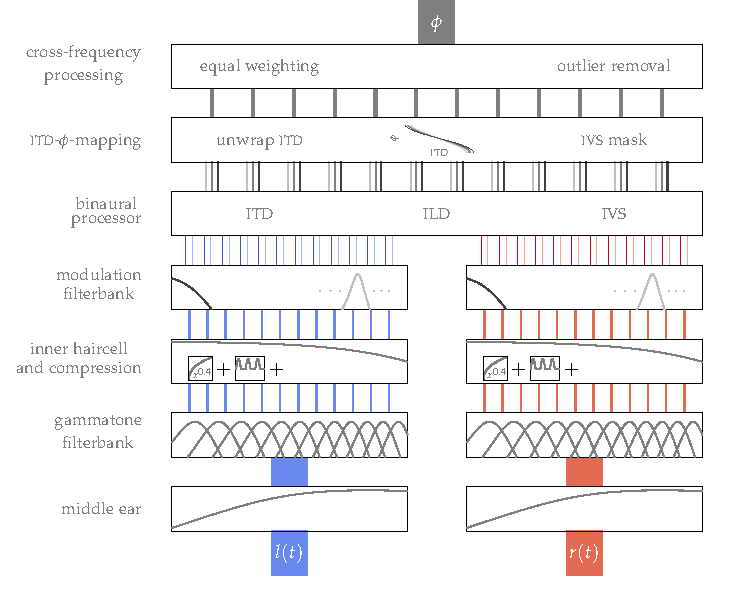
\includegraphics{fig6_01/fig6_01}
    \caption{Sketch of the applied binaural model.
    At the bottom the two time signals $l(t)$ and $r(t)$ are the input to the
    model. After that identical monaural preprocessing is applied. The binaural
    processor calculates the \ac{ITD}, \ac{ILD}, and \ac{IVS} based on the
    arriving input signals for every frequency channel. At the end the binaural
    parameter is mapped to a single direction estimation averaged over the whole
    time of the input signals.
    \reproduce{\GITHUB/fig6_01}
    \label{fig:sketch_dietz_model}}
\end{figure}
%
%\urlnote{dietz2011.m}{\AMT/binaural/dietz2011.m}
%\urlnote{wierstorf2013estimateazimuth.m}{\AMT/modelstages/wierstorf2013estimateazimuth.m}

The binaural model applied in this thesis piggybacks on the model presented by
Dietz et al.\autocite{Dietz2011} that bases its procedure on the rate coding of
the \ac{IPD}. First, the detailed processing steps applied in this thesis will be
described. Afterwards differences to the original model are discussed. The general
structure of the model consists of the following steps and is depicted in
Figure\,\ref{fig:sketch_dietz_model}:
%\marginnote[0.1cm]{\url{dietz2011.m}{\AMT/binaural/dietz2011.m}}
%\marginnote[0.1cm]{\url{wierstorf2013estimateazimuth.m}{\AMT/modelstages/wierstorf2013estimateazimuth.m}}
\begin{itemize}
    \item The middle ear transfer characteristic is approximated by a
        \marginnote[-4.5cm]{\url{dietz2011.m}{\AMT/binaural/dietz2011.m}}
        \marginnote[-4cm]{\url{wierstorf2013estimateazimuth.m}{\AMT/modelstages/wierstorf2013estimateazimuth.m}}
        first-order band-pass filter between $500$\,Hz and
        $2$\,kHz.\autocite{Puria2003}
    \item The auditory filters present at the basilar membrane are modeled with
        a fourth-order gammatone-filterbank.\autocite{Hohmann2002}
        Twelve filter bands were applied in the range of $200$\,Hz to $1400$\,Hz
        with a spacing of $1$\,ERB.
    \item Compression of the cochlea was
        modelled as to the power of $0.4$.\autocite{Ewert2000,Ruggero1997}
        The transduction process of the inner
        hair-cells was implemented with a half-wave rectification followed by a
        successive 770\,Hz fifth-order low-pass filter.\autocite{Breebaart2001}
    \item The signals leaving the haircell stage have a DC component and are
        broaden in frequency. To derive a meaningful phase difference a second
        stage of bandpass filtering has to be applied. This is done by a
        gammatone filterbank with second-order filters with an attenuation of
        $10$\,dB. Every filter is centered at the corresponding center frequency
        of the twelve frequency channels. In addition a second-order low-pass
        filter with a cutoff frequency of $30$\,Hz is applied to every frequency
        channel in order to calculate the \ac{ILD}.
    \item At the output of the band-pass filter the interaural transfer function
        is calculated in order to derive the \ac{IPD} from it. The
        \ac{IPD} is then divided by the instantaneous frequency for getting the
        \ac{ITD}. To be able to estimate the reliability of the binaural
        parameters at certain time-frequency steps the \ac{IVS} is derived as an
        approximation of the interaural
        coherence.\sidenote[][-3.7cm]{\cite[Compare][]{Faller2004,Goupell2006}}
    \item The sign of the \ac{ILD} in each frequency channel is a way to extend
        the $\pi$-limit of the \ac{IPD} to $2\pi$ which gives the opportunity to
        get the natural range of \acp{ITD} between $-700$\,ms and $+700$\,ms.
        This way center frequencies up to $1.4$\,kHz can be handled. This process is called
        \emph{unwrapping} the \ac{ITD}. For details see Figure\,2
        in Dietz et al.\autocite{Dietz2011} and the corresponding discussion.
    \item A lookup table with stored \ac{ITD} values and the
        corresponding azimuth angles converts the \ac{ITD} in the perceived
        direction in each frequency channel and for every time sample.
        The lookup table was generated with the same \ac{HRTF} set the
        binaural synthesis utilizes and has a resolution of $1\degree$.
    \item An \ac{IVS} binary mask is created by setting the threshold of the
        \ac{IVS} value to $0.98$ and
        demanding a rising slope condition with
        $\frac{\text{dIVS}(t)}{\text{d}t} \ge 0$. The median over time
        of the direction is then calculated in every frequency channel by using
        only those time steps that are fullfilling the conditions of the binary
        \ac{IVS} mask.
    \item Eventually the median over the direction in the single frequency
        channels is
        calculated. If the azimuth of single frequency bands deviate more
        than $30\degree$ from the median these frequency bands are removed and
        the median is recalculated. The median azimuth is then the
        provided estimation for the direction of the auditory event corresponding
        to the two ear signals from the beginning.
\end{itemize}

For the last step of the model a weighting of the directions in the different
frequency bands is possible. For example,
Raatgever\autocite[][Sec.\,3.4]{Raatgever1980} has found large differences
in the degree single frequency bands dominate the perceived lateralization in
the presence of conflicting cues in different frequency bands. Dietz et
al.\autocite{Dietz2011} applied a weighting accordingly to the magnitude of the
signal in the different frequency bands. In this thesis both weighting
methods were tested, but both impaired the results compared to an equal
weighting scheme. Especially the strong weighting after the data by Raatgever
leads to large deviations of the model predictions compared to the
localization results from the listening experiments.
Therefore, an equal weighting of the different frequency bands was adopted for
this thesis. This is also in accordance with the results for modelling listening
data from stereophonic experiments presented in
Park.\autocite[][Fig.\,5.10]{Park2007}

For predicting the directions of up to five different speakers the study by
Dietz et al.\autocite{Dietz2011} also utilizes the \acp{IPD} of the envelope
signal for frequency channels above $1.4$\,kHz. They found that these \ac{IPD}
cues were not as salient as the ones derived from the fine structure at lower
frequency channels and were not able to improve the results by including them.
In a similar way the performance of the binaural model could not be enhanced by
including these envelope \acp{IPD} for the prediction of the localization of
synthesized sources in this thesis. Therefore, they will be considered neither in the
following nor included in the description of the applied
binaural model.


%%%%%%%%%%%%%%%%%%%%%%%%%%%%%%%%%%%%%%%%%%%%%%%%%%%%%%%%%%%%%%%%%%%%%%%%%%%%%%%%
\section{Validation of the Binaural Model}
\label{sec:validation_of_the_binaural_model}
%
The binaural model described in the last section was validated by all of the
data from the listening experiments presented in Section\,\ref{sec:localization}.
In addition to the perceived direction the localization blur was estimated by
the standard deviation of the azimuth value of the model over time.
The five repetitions of every condition for each listener were simulated by
applying five different noise bursts to the model. Afterwards the mean about
these five stimuli were calculated for the predicted direction and its
corresponding localization blur.
In addition, eleven listeners were simulated by applying different head
orientations of the binaural model. For the first listener the model was facing
the secondary sources forward at $0\degree$. The second listener was facing
towards $1\degree$ and so forth. The offset in the perceived angle due to the
head orientation was compensated for in the estimation of the direction of the
synthesized source. Afterwards the mean and confidence values were calculated
above the eleven different head orientations for both the direction and
localization blur, given by the standard deviation for single head orientation.

In exactly the same way as for the data from the listening experiment, the
prediction data of the binaural model was inspected for deviations from a
single Gaussian distribution. For cases were the data could not be explained by
a single distribution a Gaussian mixture model was applied to separate the data
into two distributions -- compare
Figure\,\ref{fig:model_localization_distribution} and
\ref{fig:localization_distribution}.
%
\begin{figure}
    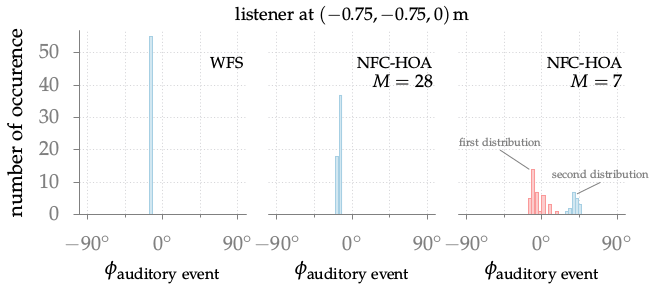
\includegraphics{fig6_02/fig6_02}
    \caption{Distributions of the auditory event's directions as predicted
    by the binaural model for the listening position $(-0.75,-0.75,0)$\,m and the
    circular secondary source distribution with 14 sources.
    The results for a synthesized point source for \ac{WFS} and
    \ac{NFC-HOA} up to different orders $M$ are shown.
    \reproduce{\GITHUB/fig6_02}}
    \label{fig:model_localization_distribution}
\end{figure}


\renewcommand{\thefigure}{\thechapter.\arabic{figure}a} % add a to figure number
\begin{figure}
    \centering
    \hspace*{-1.2cm}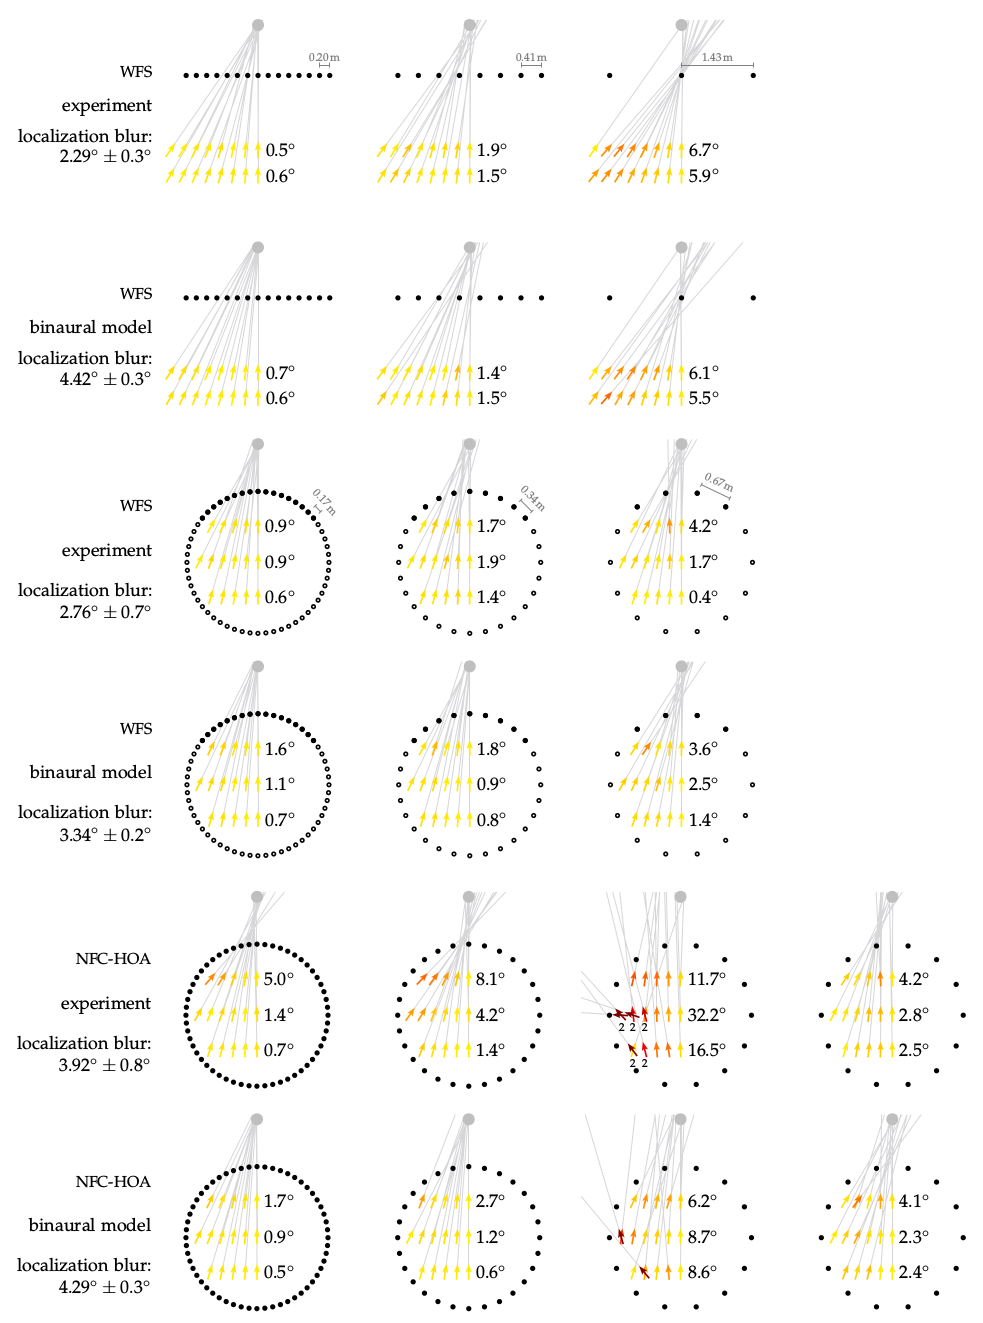
\includegraphics{fig6_03/fig6_03a}
    \caption{Average localization results for all four experiments. The black
    symbols indicate loudspeakers, the grey ones the synthesized source. On
    every listening position an arrow is pointing into the direction the
    listener perceived the corresponding auditory event from. The color of the arrow
    displays the absolute localization error, which is also summarized beside
    the arrows for every row of positions. The average confidence interval for
    the localization results is $2.3\degree$. Listening conditions that
    resulted in listeners saying that they perceived two sources in Exp.\,4 of
    Section\,\protect\ref{sec:localization} are
    highlighted with a small $2$ written below the position.
    \reproduce{\GITHUB/fig6_03}}
    \label{fig:localization_results_model}
\end{figure}
%
\renewcommand{\thefigure}{\thechapter.\arabic{figure}b} % add b to figure number
\begin{figure}
    \ContinuedFloat % needs the subfig package
    \centering
    \hspace*{-1.2cm}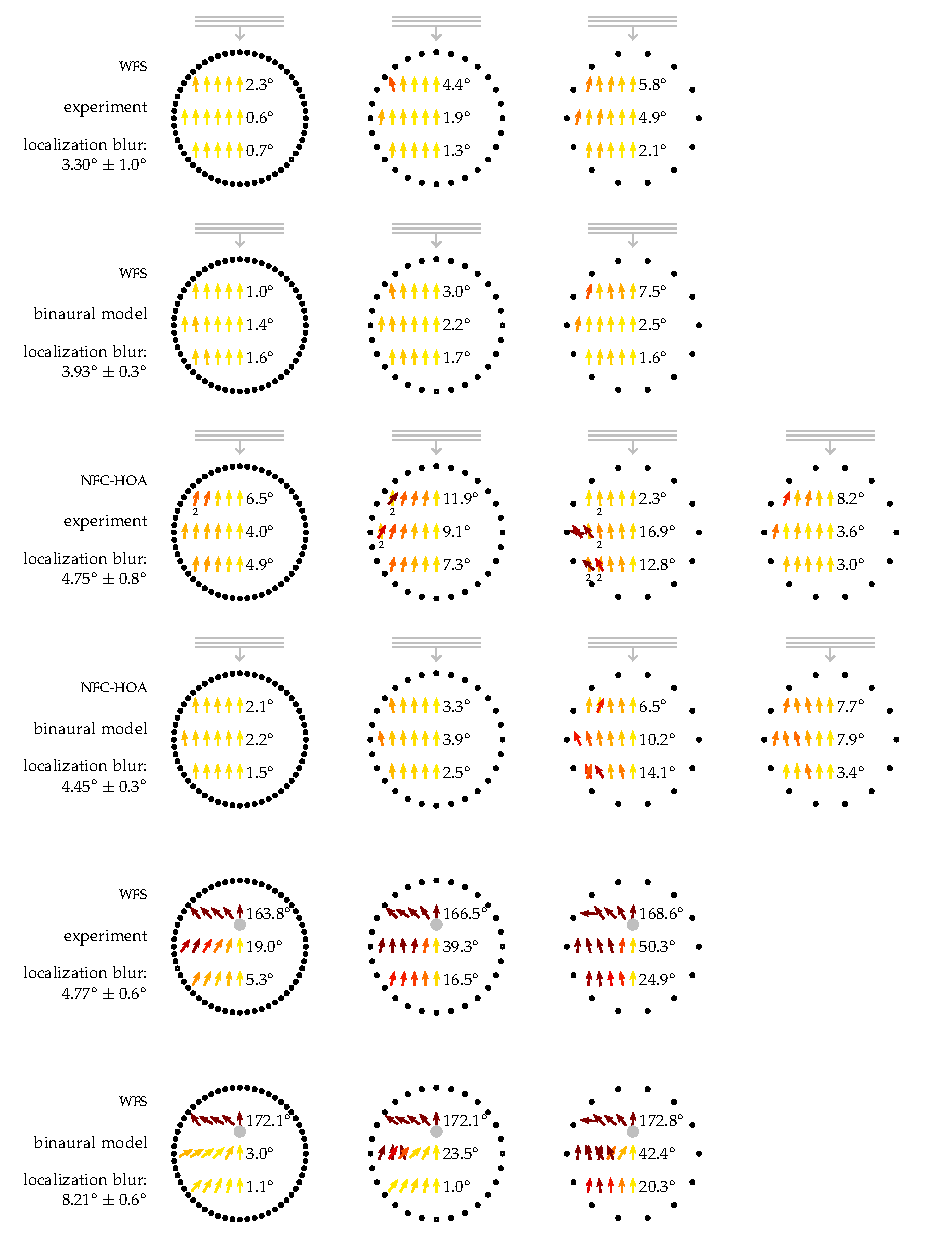
\includegraphics{fig6_03/fig6_03b}
    \caption{Average localization results for all four experiments. The black
    symbols indicate loudspeakers, the grey ones the synthesized source. On
    every listening position an arrow is pointing into the direction the
    listener perceived the corresponding auditory event from. The color of the arrow
    displays the absolute localization error, which is also summarized beside
    the arrows for every row of positions. The average confidence interval for
    the localization results is $2.3\degree$. Listening conditions that
    resulted in listeners saying that they perceived two sources in Exp.\,4 of
    Section\,\protect\ref{sec:localization} are
    highlighted with a small $2$ written below the position.
    \reproduce{\GITHUB/fig6_03}}
    \label{fig:localization_results_model}
\end{figure}
\renewcommand{\thefigure}{\thechapter.\arabic{figure}} % restore normal figure numbering
%
\newthought{All model predictions} are compared with all localization results
from the experiments in Figure\,\ref{fig:localization_results_model}.
The figure visualizes that the model predictions are very accurate, especially for the
case of \ac{WFS} and a synthesized point source or plane wave. By averaging the
results for all these conditions the deviation of the model results from the
experimental data is $1.8\degree$ with the largest deviation being $14\degree$ 
for 14 secondary sources and a synthesized plane wave at the listener position
$(0.75,-0.5,0)$\,m.

The problem of more than one perceived source was
ignored for testing the model performance by assuming a single perceived source
at all positions. Therefore, the mean value of both directions for
these cases was used. The accuracy of the model predictions is then in average $8\degree$
for all \ac{NFC-HOA} conditions. Whereby the model performance is slightly
better for a synthesized point source and higher orders. The maximum deviation
is $40\degree$ for a secondary source distribution with 14 sources and an
order of 7 for the spherical harmonics at the listener position of $(-1.25,0,0)$\,m.
For the focused source condition and \ac{WFS} the model predicted a correct
localization of the synthesized source even for several positions were the listener
had large deviations.
That leads to the largest deviations of the model prediction from the
experimental data for focused sources of $11\degree$ in average. The maximum
deviation was $40\degree$ for a secondary source distribution of 28 sources and
the listener position $(-0.5,0,0)$\,m.

Beside the perceived direction the localization blur was modeled by calculating
the standard deviation of the predicted direction over time.
This method could predict the localization blur adequately when averaging
over the different loudspeaker arrays. Looking at the single loudspeaker array
the localization blur of the model depended on the number of used loudspeaker,
having a larger localization blur for the arrays with fewer loudspeakers. In the
listening experiment no such dependency could be observed.

\newthought{The most interesting} conditions are those where the model is not
as accurate as for the other ones. Especially the case for focused sources is
challenging. For a closer inspection of the model behavior
for these cases the \ac{ITD} values for different frequencies
channels over time will be analyzed. Figure\,\ref{fig:itd_frequency_channels}
visualizes them for a listener position of $(-0.75,0,0)$\,m. The top row presents
the situation of \ac{WFS} and a focused source. The \acp{ITD} of three adjacent
frequency channels are plotted in the same color.
\acp{ITD} for frequencies
around $200$\,Hz are marked as blue points, \acp{ITD} for frequencies around
$500$\,Hz as green, $800$\,Hz as yellow, and $1200$\,Hz as red.
%
\begin{figure}
    \centering
    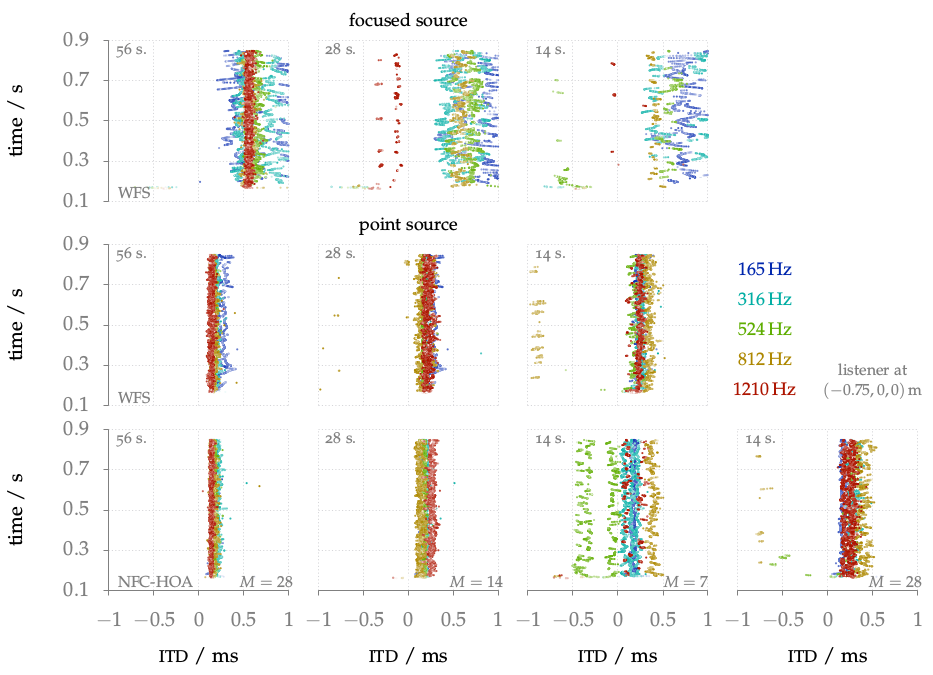
\includegraphics{fig6_04/fig6_04}
    \caption{\ac{ITD} values over time for different frequencies as indicated by the
    color. The \ac{ITD} was calculated by the binaural model for a single noise
    burst synthesized as a focused source or point source with
    \ac{WFS}~\protect\eqref{eq:d_wfs_fs_25D}, \protect\eqref{eq:d_wfs_ps_25D} and
    \ac{NFC-HOA}~\protect\eqref{eq:D_nfchoa_ps_25D}.
    The magnitude of the signal in the frequency channel is indicated by the
    opacity of the \ac{ITD} points, with lighter points correspond to
    lower magnitudes.
    \reproduce{\GITHUB/fig6_04}}
    \label{fig:itd_frequency_channels}
\end{figure}
%
For a secondary source distribution with 56 sources the \acp{ITD} are clustered
around $-0.6$\,ms, whereby the lower frequencies are spread in a larger region
ranging from $-0.2$\,ms to $1$\,ms. This is not astonishing, because the
minimal size of the focal point is determined by its wave length. For example,
a frequency of $240$\,Hz corresponds to a size of $1.4$\,m of the focal
point. For the two secondary source distributions with less sources the
\acp{ITD} for lower frequencies are still spread out in the same area, but those
for higher frequencies are vanishing or have negative values.
Comparing this with the listener results it is of interest that the listeners
perceived the focused source to come from the left for the secondary source
distributions with 14 and 28 sources, whereby the model predicted them to come
from the right and the left. The latter was a result of including different
head orientations. Figure\,\ref{fig:itd_frequency_channels} shows only the head
orientation of $0\degree$ for which the perceived direction would be predicted
to come from the right for 14 and 28 sources.

Beside \acp{ITD} for focused sources, Figure\,\ref{fig:itd_frequency_channels}
furthermore compares the \acp{ITD} for a point source synthesized with \ac{WFS} and
\ac{NFC-HOA}. The localization accuracy of the listener was around $1\degree$ for
\ac{WFS} in the listening experiment at the corresponding listening position of
\linebreak
$(-0.75,0,0)$\,m. Whereas, for \ac{NFC-HOA}
the accuracy was around $3\degree$ for all conditions with $M>7$.
For an order of $M=7$ and 14 secondary sources the listener reported to
perceive two sources. The binaural model was not able to predict the two
sources for that condition. However, the corresponding \ac{ITD} values indicate at least
that the localization should be significantly different from the corresponding
\ac{WFS} condition as they are spread for some frequencies in the negative and
positive region.
These differences point out that the performance of the binaural model probably
could be improved for the challenging conditions.


%%%%%%%%%%%%%%%%%%%%%%%%%%%%%%%%%%%%%%%%%%%%%%%%%%%%%%%%%%%%%%%%%%%%%%%%%%%%%%%%
\section[Example Applications of the Binaural Model]{Example Applications of the
Binaural Model in Sound Field Synthesis}
\label{sec:model_applications}

The last section validated the predictions of the binaural model
and highlighted its limits. This section will present some example applications
of the binaural model in the context of sound field synthesis.
It will be predicted how the localization is in the audience area. Another
question is for which setups the listener will localize the synthesized sources
towards the direction of the nearest loudspeaker.
In addition, the model can be employed as a planing tool by specifying the
size of the sweet-spot that a setup should achieve.

%--%--%--%--%--%--%--%--%--%--%--%--%--%--%--%--%--%--%--%--%--%--%--%--%--%--%-
\subsection{Prediction of Localization for Sound Field Synthesis and Arbitrary
Secondary Source Distributions}
\label{sec:prediction_of_localization_for_sound_field_synthesis_and_arbritrary_setups}
%
The validation of the binaural model has shown that the model is especially
able to predict the localization for \ac{WFS} with high accuracy. Hence, the model can
be used to predict the localization accuracy for \ac{WFS}
in the whole audience area. Figure\,\ref{fig:wfs_linear_model} shows the
estimations of the perceived direction for the same setup that was applied in
the experiment in Section\,\ref{sec:localization}. However, this time the audience area
was sampled with a higher resolution of around $15$\,cm.
%
\begin{figure*}
    \centering
    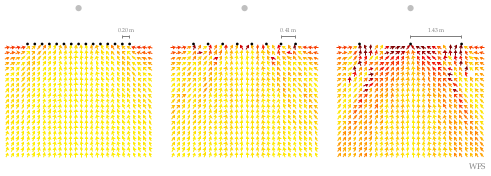
\includegraphics{fig6_05/fig6_05}
    \caption{Model predictions of the perceived directions for a synthesized point
    source in the audience area. The three different linear secondary source
    distributions were all driven by \ac{WFS}~\protect\eqref{eq:d_wfs_ps_25D}.
    \reproduce{\GITHUB/fig6_05}}
    \label{fig:wfs_linear_model}
\end{figure*}
%
The model predictions support the results of the listening test. The
localization is not impaired by \ac{WFS} and a distance between the secondary
sources of $20$\,cm. In this case the absolute localization error averaged over
all listening positions is $1.6\degree$. 
By doubling the distance the localization accuracy slightly becomes
degraded, but still is relatively equal in the whole audience area. The
average absolute localization error is now $3.4\degree$.
Whereas the setup with 3 secondary sources leads to an average absolute
localization error of $10.3\degree$ and the localization of
the nearest loudspeaker at several listener positions.
The ratio between localising single loudspeaker or the synthesized source is
further analyzed in the next section.

The model furthermore gives the opportunity to test the influence of different
secondary source geometries on the localization results.
Figure\,\ref{fig:wfs_model} summarizes the result for two different geometries.
%
\begin{figure}
    \centering
    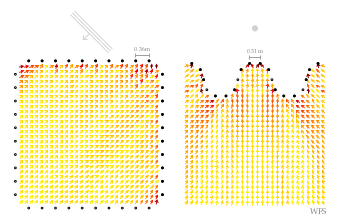
\includegraphics{fig6_06/fig6_06}
    \caption{Model predictions of the perceived direction for a synthesized
    sources in the audience area. Both secondary source
    distributions were driven by \ac{WFS} with~\protect\eqref{eq:d_wfs_pw_25D} for the
    plane wave and~\protect\eqref{eq:d_wfs_ps_25D} for the point source.
    \reproduce{\GITHUB/fig6_06}}
    \label{fig:wfs_model}
\end{figure}
%
In the left of the figure a box shaped secondary source distribution was applied.
This geometry is of special interest, because it can easily be installed in
rooms and was among the first ever build \ac{WFS}
setups.\sidenote[][-0.1cm]{\cite[For an overview of existing \ac{WFS} systems
see][]{DeVries2009}}
If a source is coming from a direction orthogonal to one of the four linear
parts of the distribution the perception will be similar to a linear source
distribution. Of high interest are those synthesized sources coming from the direction
of the array's edges. In Figure\,\ref{fig:wfs_model} a plane wave with an
incidence direction of $(-1,-1,0)$ is synthesized. The model predictions
indicate
that the localization accuracy in this case is only impaired directly in the
edges of the array and comparable to the one of a linear array at all other
positions within the audience area.

The second example employs a smaller version of the concave secondary source
distribution from Figure\,\ref{fig:concave_array}.
The prediction results of the binaural model show that the
concave parts introduce an impairment of the localization
accuracy especially in the proximity of the secondary sources. 

\newthought{Comparing the} model predictions the accuracy for \ac{NFC-HOA} was
not as convincing as for \ac{WFS}. Nonetheless, as long as the order of the
\ac{NFC-HOA} systems was $14$ or above the results were in fair agreement with
the listening tests.
Therefore, the binaural model will only be applied for \ac{NFC-HOA} with orders
of $14$ in the following.
An interesting question in the context of \ac{NFC-HOA} is the vulnerability of
the system to variations of the secondary source distribution from a perfect
circle as the underlying theory assumes.
Figure\,\ref{fig:nfchoa_model} shows results for a perfect
circular geometry, an impaired one that has different angles between the single
sources, and an impaired one that has a random jitter of up to $7$\,cm on
its source positions. For the different angles a circular secondary source
distribution with 56 sources was created and randomly 28 of those sources were
chosen.
%
\begin{figure*}
    \centering
    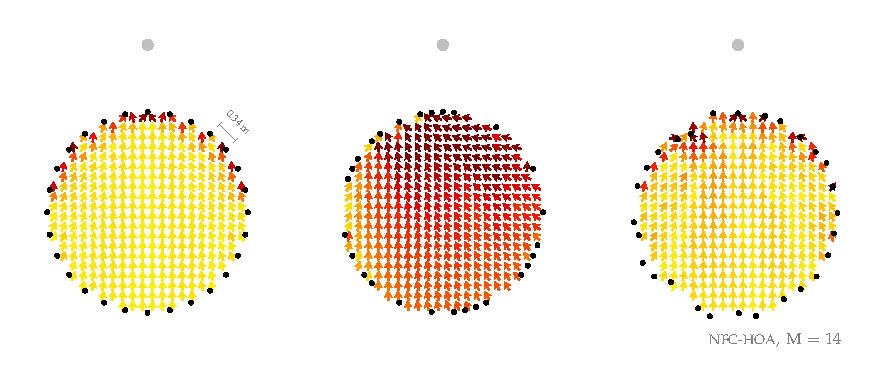
\includegraphics{fig6_07/fig6_07}
    \caption{Model predictions of the perceived direction for a synthesized
    point source in the audience area. All three secondary source distributions
    were driven by \ac{NFC-HOA}~\protect\eqref{eq:D_nfchoa_ps_25D} with an order of
    $14$. For both distributions to the right the positions of the secondary
    sources were changed.
    \reproduce{\GITHUB/fig6_07}}
    \label{fig:nfchoa_model}
\end{figure*}
%
The results for the regular distribution show very high
localization accuracy. In fact, compared to the results from the listening test
in Figure\,6.3 the model probably predict a too
high localization accuracy.
If the angles between the single secondary sources are varied the overall localization
accuracy drops enormously. Further investigation reveals that the position of
the synthesized source is shifted to the left. Considering this shift the
localization accuracy is only slightly impaired. Such a shift can occur if the
secondary sources are not equally distributed on the circle as the underlying
driving functions assume. In the given example they are
more dense at the right bottom and left top of the distribution.
The results for the randomly jittered secondary sources are presented in the
right graph of Figure\,\ref{fig:nfchoa_model}. They show that slight variations
of the secondary source positions can influence the localization of
the synthesized source. At listening positions to the side the localization is
now more towards the frontal sources of the distribution than towards the
synthesized source. 


%--%--%--%--%--%--%--%--%--%--%--%--%--%--%--%--%--%--%--%--%--%--%--%--%--%--%-
\subsection{Determining the Border of Single Loudspeaker Localization}
\label{sec:determinig_the_border_of_single_loudspeaker_localization}
%
The sweet-spot phenomenon for stereophony implicates that outside
of the sweet-spot listener get the impression that the auditory events come from
the nearest loudspeaker. An unsettled question is how
many loudspeakers are needed for a linear secondary source distribution in
\ac{WFS} in order to avoid the localization of single loudspeakers as it is for
example the case for a loudspeaker array with 3 sources as presented in
Figure\,\ref{fig:wfs_linear_model}.
One way of measuring is to predict the perceived direction with the binaural
model at every listener position similar to Figure\,\ref{fig:wfs_linear_model} and
afterwards calculate if the perceived direction is closer to the actual position of the
synthesized source or the nearest loudspeaker. After performing the prediction for
each position the ratio between loudspeaker and synthesized source localization
could be calculated over all listener positions.

The calculation conducted for the same \ac{WFS} configuration as shown in
Figure\,\ref{fig:wfs_linear_model} for 2, 3, 4, up to 16 secondary sources.
For only 2 secondary sources the listener localizes towards the nearest
secondary source at $90\%$ of all positions in the audience area.
Using 3 secondary sources this is only the case for $40\%$ of all positions,
using 4 secondary sources for $10\%$ of all
positions and for 8 secondary sources it vanishes completely.


%--%--%--%--%--%--%--%--%--%--%--%--%--%--%--%--%--%--%--%--%--%--%--%--%--%--%-
\subsection{Estimating the Size of the Sweet-Spot}
\label{sec:estimating_the_size_of_the_sweet_spot}
%
In the introduction of this thesis the phenomenon of the sweet-spot in stereophony was
discussed and sketched in Figure\,\ref{fig:stereophony}. Normally in stereophony
this term combines two facts: the existence of a small area in which the
localization behaves as wanted and localization of the nearest loudspeaker
outside of this area. As discussed in the last section the
localization of single loudspeaker in \ac{WFS} only happens for
secondary source distributions consisting of less than 4 loudspeakers.
Extending the idea of the sweet-spot to \ac{SFS} it is defined
as a first approximation to be that part of the audience area where
the localization accuracy is equal or better than a given value.

The localization accuracy was calculated by the binaural model for different
\ac{SFS} setups and stereophony. Figure\,\ref{fig:sweet-spot-size} summarizes
the results by coloring all parts of the audience area that give a
localization accuracy of $5\degree$ or better in blue.
The result replicates the small sweet-spot of stereophony. In addition,
the sweet-spot extends towards the whole audience area for \ac{WFS}, achieving the
desired effect shown in the introduction in Figure\,\ref{fig:stereophony}.
It further demonstrates that a \ac{WFS} system and a
\ac{NFC-HOA} system without band-limitation yield an identical spatial
impression.
%
\begin{figure}
    \centering
    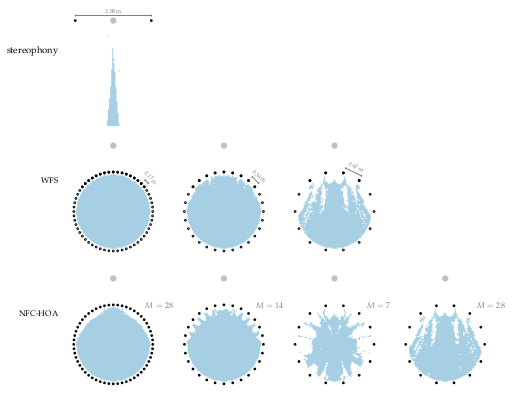
\includegraphics{fig6_08/fig6_08}
    \caption{Model prediction of the sweet-spot sizes for different \ac{SFS}
    setups synthesizing a point source. As a comparison a stereophony setup
    presents the same source.
    The sweet-spot is defined as all points where the absolute localization error
    is less or equal to $5\degree$.
    \reproduce{\GITHUB/fig6_08}}
    \label{fig:sweet-spot-size}
\end{figure}

\newpage

For band-limited \ac{NFC-HOA} the spread of the sweet-spot for the two
distributions with less secondary sources shows that the localization is getting
wrong in the proximity of the single loudspeakers.
What cannot be directly concluded from the sweet-spot sketch is to which extent
the localization will be impaired outside of the sweet-spot.
The results of the listening experiment have shown that severe problems can occur
for band-limited \ac{NFC-HOA}.
In that case even more than one auditory event could be perceived outside of the sweet-spot.


%%%%%%%%%%%%%%%%%%%%%%%%%%%%%%%%%%%%%%%%%%%%%%%%%%%%%%%%%%%%%%%%%%%%%%%%%%%%%%%%
\section{Summary}
\label{sec:modelling_summary}
%
A binaural model after Dietz et al.\autocite{Dietz2011} was modified and
validated against the localization results from Section\,\ref{sec:localization}.
The model showed very good agreement with the test results, especially in the
case of \ac{WFS} and \ac{NFC-HOA} with high orders. For band-limited \ac{NFC-HOA}
the model had to be extended, because listeners reported perceiving more than
one auditory event outside the sweet-spot. This was accomplished by the
usage of different head-orientations during the prediction of the localization.
Afterwards, a Gaussian mixture model helped to identify the different directions.

For focused sources synthesized with \ac{WFS} the model is not able
to predict the localization of focused sources in the whole listening area with
a high accuracy. It performed better in the localization task of
the synthesized source than the listeners.
By inspecting \acp{ITD} for different frequency channels the model still allows
interesting discernments.

Towards the end of the chapter the validated model was used for some example
applications like predicting the size of a sweet-spot. These applications
highlight the value a binaural model could have for planing new loudspeaker array
setups for \ac{SFS} or comparing different \ac{SFS} approaches.
